\documentclass[ignorenonframetext]{beamer}

%\documentclass[handout,ignorenonframetext]{beamer}

% Standardni paketi:
\usepackage[slovene]{babel}
\usepackage[utf8]{inputenc}
\usepackage[T1]{fontenc}
\usepackage{lmodern}
\usepackage{amsmath}

% Paketi, s katerimi določimo željene pisave:
\usepackage{mathptmx}
\usepackage{helvet} % splošen font pisave
\usepackage{courier} %font pisave v okolju verbatim

% Kot v article lahko definiramo nova okolja:
\newtheorem{definicija}{Definicija}
\newtheorem{izrek}{Izrek}
\newtheorem{zgled}{Zgled}
\newtheorem{opomba}{Opomba}
\newcommand{\norm}[1]{\left\lVert#1\right\rVert}

\mode<article>{
\setlength{\parindent}{0cm}
\usepackage{amsfonts}
\let\frametitle\subsection %%naslovi slidov postanejo naslovi podrazdelkov v article
}

\mode<beamer>{
\usetheme{Rochester}}

\mode<handout>{
\usetheme{AnnArbor}

\useoutertheme{infolines} %določi glavo in nogo
\setbeamercovered{transparent} %neodkriti tekst je rahlo viden
\setbeamercolor{background canvas}{bg=black!5}
\usepackage{pgfpages} %2 na 1 stran
\pgfpagesuselayout{2 on 1}[a4paper, border shrink=5mm]
}

\title{Spojena kubična Bezierjeva krpa}
\author{Matija Šteblaj, Nejc Ševerkar}
\date{14. 1. 2021}

\begin{document}

\begin{frame}
\titlepage
\end{frame}

\begin{frame}
\frametitle{Aproksimacija parcialnih odvodov}

Naš vhodni podatek so le točke v prostoru, ker pa smo v metodi predpostavili 
poznavanje parcialnih odvodov v vsaki od teh točk, moramo te oceniti.
\vspace{10px}
Recimo, da imamo dane točke
$$P = (p_i)_i = (x_i,y_i,z_i)$$
in ocenjujemo parcialna odvoda v testni točki $p_k$.
\end{frame}

\begin{frame}
\frametitle{1. Korak}
Odvoda v $p_k$ bomo ocenili s pomočjo točk v neki njeni okolici. 
In sicer določimo radij $r_k$ in obravnavajmo točke $p_j \in P$ za katere $d((x_j,y_j), (x_k,y_k)) = d^k_j < r_k$.
Recimo, da so indeksi teh $1,\dots, n_k$.
\begin{center}
	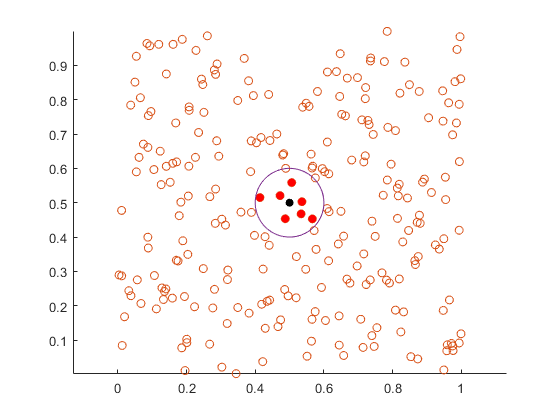
\includegraphics[width=230px]{slike/pointRadius.png}
\end{center}
\end{frame}

\begin{frame}
\frametitle{2. Korak}
S formulo 
$$w^k_j = (r_k - d^k_j) / (r_k \cdot d^k_j)$$
je definirana utež točke $p_j$, ki izraža njen vpliv na odvod testne točke $p_k$.
Ideja je spet ta, da so točke bližje $p_k$ bolj utežene, saj nam o odvodu povejo več.
\end{frame}

\begin{frame}
\frametitle{3. Korak}
Definiramo interpolacijski polinom za $p_k$, stopnje $2$ in dveh spremenljivk
\begin{equation*}
\begin{aligned}
p(x,y) &= z_k + a \cdot (x - x_k)^2 + b \cdot (x - x_k) \cdot (y - y_k) \\
&+ c \cdot (y - y_k)^2 + d \cdot (x-x_k) + e\cdot(y-y_k),
\end{aligned}
\end{equation*}
kjer so $a,b,c,d,e,$ nedoločeni členi in velja 
$$p_x(x_k,y_k) = d \quad \text{in} \quad p_y(x_k,y_k) = e.$$
\end{frame}

\begin{frame}
\frametitle{3. Korak}
Naravno si želimo, da bi ta polinom dobro aproksimiral vrednosti $z_j$ za $j = 1, \dots, n_k$. Minimiziramo torej
$$\sum_{j =1}^{n_k} (w^k_j \cdot (p(x_j,y_j) - z_j))^2 = \norm{W_kAu - W_kv}^2,$$
kjer je $u = [a,b,c,d,e]^T$ iskan vektor, $A$ matrika
\begin{equation*}
\begin{vmatrix}
(x_1 - x_k)^2 &  (x_1 - x_k) (y_1 - y_k) & (y_1 - y_k)^2 & (x_1 - x_k) & (y_1 - y_k) \\
(x_2 - x_k)^2 &  (x_2 - x_k) (y_2 - y_k) & (y_2 - y_k)^2 & (x_2 - x_k) & (y_2 - y_k) \\
\vdots & \vdots & \vdots & \vdots & \vdots \\
(x_{n_k} - x_k)^2 & (x_{n_k} - x_k) (y_{n_k} - y_k) & (y_{n_k} - y_k)^2 & (x_{n_k} - x_k) & (y_{n_k} - y_k)
\end{vmatrix},
\end{equation*}
$W_k = \text{diag}(w^k_1, w^k_2, \cdots, w^k_{n_k})$ ter $v = [z_1 - z_k, \cdots, z_{n_k} - z_k]^T$.
\end{frame}

\begin{frame}
\frametitle{3. Korak}
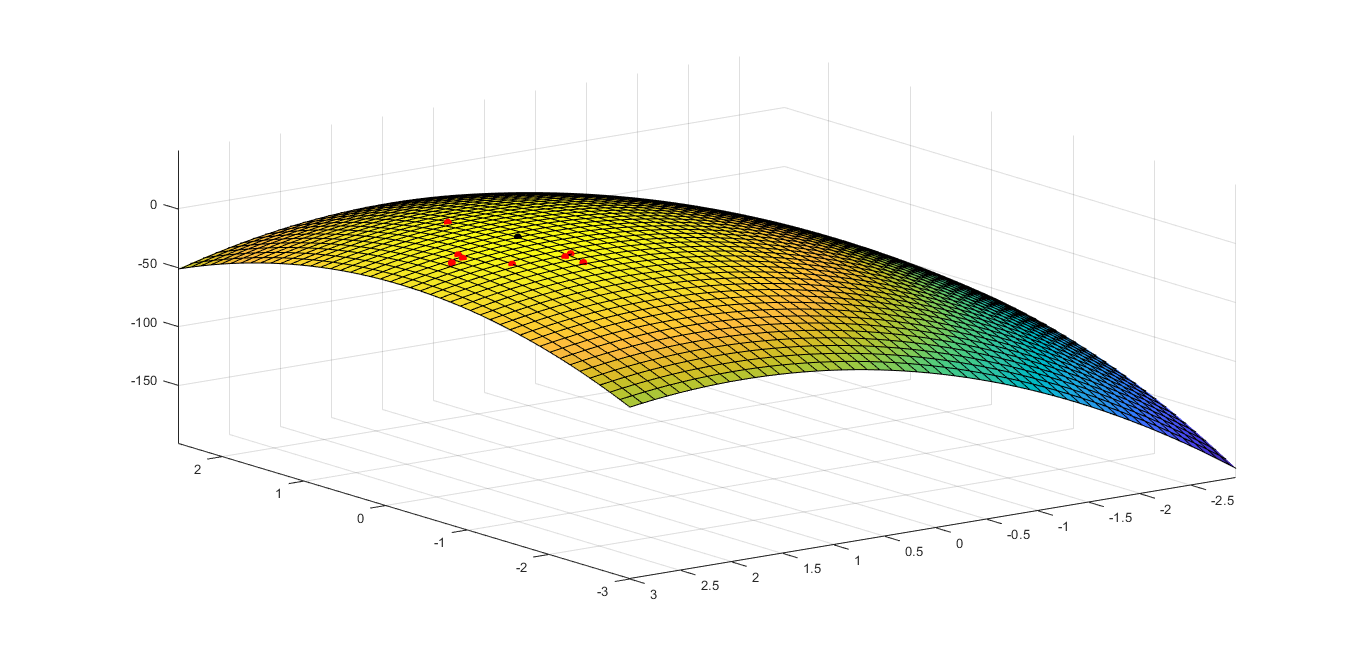
\includegraphics[width=\textwidth, height=\textheight]{slike/surfInterpol.png}
\end{frame}

\begin{frame}
\frametitle{Aproksimacija razsevnih podatkov}
Radi bi aproksimirali neko množico točk $P$ v prostoru s shemo, ki smo jo predstavili prej.
Konstrukcija poteka v treh korakih
\begin{enumerate}
\item V vsaki točki $p_k$ ocenimo parcialne odvode
\item Trianguliramo točke $(x_i,y_i)_i$
\item Na vsakem trikotniku $T$ konstruiramo lokalno shemo z metodo Goodman-Said in shranimo matriko 
\begin{equation*}
B_T = 
\begin{vmatrix}
b_{300} & b_{210} & b_{120} & b_{030} \\
b_{201} & \openbox & b_{021} & \openbox  \\
b_{102} & b_{012} & \openbox & b_{1112} \\
b_{003} & \openbox & b_{1113} & b_{1111}
\end{vmatrix}
\end{equation*}
Podatki na vseh trikotnikih podajo našo aproksimacijo.
\end{enumerate}

\end{frame}

\begin{frame}
\frametitle{Druge sheme}
Uporabljena shema je koristna, ker zahteva le aproksimacijo drugih odvodov v danih točkah.
Pripomnimo pa, da bi z oceno drugih odvodov lahko uporabili kar Argyrisov zlepek.
\end{frame}

\end{document}